\begin{center}
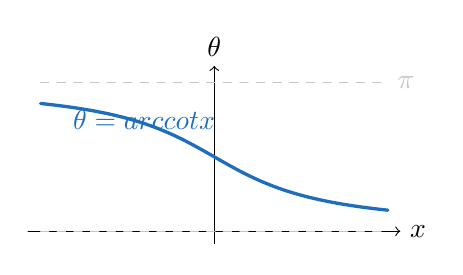
\begin{tikzpicture}[scale=1.05, line cap=round, line join=round]
  \definecolor{trigblue}{RGB}{30,110,190}
  \draw[->] (-2.25,0)--(2.25,0) node[right] {$x$};
  \draw[->] (0,-0.15)--(0,2.0) node[above] {$\theta$};
  \draw[gray!45,dashed] (-2.1,1.8)--(2.1,1.8) node[right] {$\pi$};
  \draw[gray!45,dashed] (-2.1,0)--(2.1,0);
  \draw[very thick,trigblue,domain=-2.1:2.1,samples=90]
    plot ({\x},{0.9+0.9*(-atan(\x)/90)});
  \node[trigblue] at (-0.85,1.35) {$\theta=\operatorname{arccot} x$};
\end{tikzpicture}
\end{center}
